\documentclass[a4paper, 12pt]{report}

%%%%%%%%%%%%
% Packages %
%%%%%%%%%%%%
\usepackage[english]{babel}
\usepackage{packages/sleek}
\usepackage{packages/sleek-title}
\usepackage{packages/sleek-theorems}
\usepackage{packages/sleek-listings}
\usepackage{hyperref}
\usepackage{listings}
\lstset{
    basicstyle=\ttfamily\small, 
    frame=single,              
    numbers=left,              
    numberstyle=\tiny,         
    keywordstyle=\bfseries,    
    breaklines=true,           
    captionpos=b,              
}
\graphicspath{ {./resources/img/} }
%%%%%%%%%%%%%%
% Title-page %
%%%%%%%%%%%%%%

\logo{./resources/pdf/logo.pdf}
\institute{Universidad Politécnica de Cartagena}
\faculty{Redes de Banda Ancha}
%\department{Department of Anything but Psychology}
\title{TAREA 2}
\subtitle{Redes MPLS con OSPF, BGP y VRF}
\author{\textit{Autor}\\André Yermak Naumenko}
%\supervisor{Linus \textsc{Torvalds}}
%\context{A long time ago in a galaxy far, far away...}
\date{\today}

%%%%%%%%%%%%%%%%
% Bibliography %
%%%%%%%%%%%%%%%%

\addbibresource{./resources/bib/references.bib}

%%%%%%%%%%
% Macros %
%%%%%%%%%%

\def\tbs{\textbackslash}

%%%%%%%%%%%%
% Document %
%%%%%%%%%%%%

\begin{document}
\maketitle
\romantableofcontents
\setcounter{section}{0}
\chapter{Introducción}

\textit{Las redes de transporte MPLS pueden utilizarse para conectar diversos sites de clientes empresariales, por ejemplo, distribuidos geográficamente. En el laboratorio de clase se ha realizado una conexión punto a punto a través de la red MPLS pero sólo era una extensión de nivel 2 transportando tramas Ethernet, es decir, la red MPLS actuaba como un simple hub de red. Sin embargo, es posible usar MPLS para conectar redes de un cliente a nivel 3, es decir transportando todas las rutas de un site a otro, y, además, separando las tablas de encaminamiento de diferentes clientes. Para transportar rutas de un extremo a otro de la red MPLS debe usar el protocolo BGP, y, para diferenciar el encaminamiento de cada cliente, VRF.La siguiente figura contiene el esquema general de red que debe realizar. Tenemos dos clientes, A y B, conectados a la red MPLS (Proveedor de la red de Transporte, Sistema Autónomo, AS65100) a través de routers Cisco. La nomenclatura indica:}

\textit{• PE: Provider-Edge router. Cada uno de los PEs tiene un site del cliente A y otro site del cliente B.}

\textit{• CE: CUSTomer-Edge router. Routers frontera del cliente en cada site y conectan con el router PE de la red MPLS del la red del proveedor, AS65100. Las redes de cada cliente en cada Site están en la figura. Por ejemplo, el Site 1 del cliente A tiene redes de usuario 172.16.1.0/24, y, 172.16.2.0/24.}

\textit{Para realizar este proyecto es recomendable hacerlo de forma progresiva, esto es, realizar cada ejercicio en el orden que se propone para llegar al resultado final. En los siguientes ejercicios, use en todos los routers el mismo IOS. Si utiliza la MV de la asignatura puede utilizar el router c7200-sp, cuyo IOS es Cisco7200-spservicesk9- mz.124-24.T6.image. Tenga en cuenta que si usa otro IOS podría no haber suficiente capacidad de proceso en su máquina para desarrollar la totalidad e este proyecto.}

\chapter{Ejercicios propuestos}

\section{\texttt{Ejercicio 1. Configurar la red de transporte: MPLS y OSPF}}

\textit{El siguiente esquema representa la red de transporte o MPLS Core y sustituye a la recuadro
central del esquema de la página anterior. No conecte ni configure aún los sites de los clientes.}

\textbf{Pregunta 1.}

\textit{Configure la red de la figura en GNS3:}

\begin{figure}[H]
	\centering
	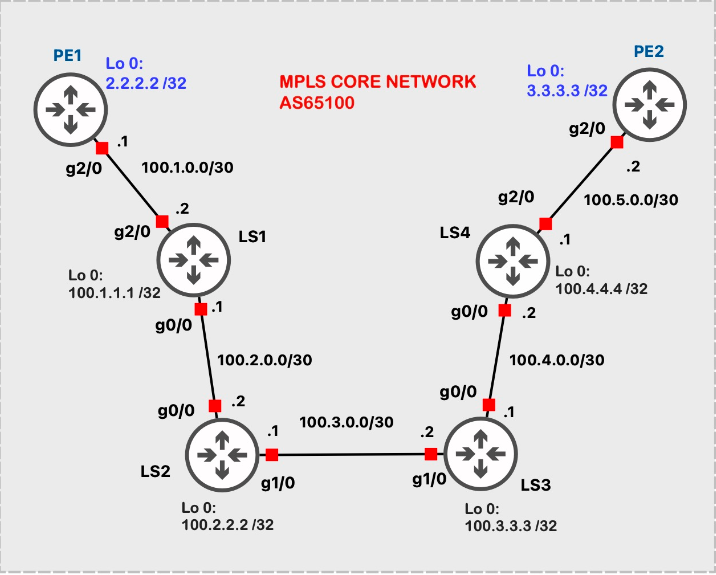
\includegraphics[scale=0.5]{maquetainicial.png}
	\caption{Fig. Red Core MPLS (AS65100).}
	\label{fig:maquetainicial}
\end{figure}

\textit{Debe, Construir la topología en GNS3 arrastrando los routers que se indican y conectarlos como se indica.}
\newpage
\textbf{Pregunta 2.}
\textit{Realice el arranque de PE1 (botón derecho sobre el router -> START) e igualmente, abra una
-> Consola. Deje que arranque el router y cambie el hostname del router a PE1. Repita la
4
Fig. Red Core MPLS (AS65100)
TAREA 2, LAB. RBA
configuración del hostname en el resto de los routers de la red, LS1, LS2, LS3, LS4, PE2.
Nota: se recomienda ir arrancando y configurando hostname de router en router.}

\textbf{Pregunta 3.}

\textit{Configurar la dirección IP de todas las interfaces. Una vez hecho, ponga en la memoria una
captura de la pantalla que muestre la red}

\begin{figure}[H]
	\centering
	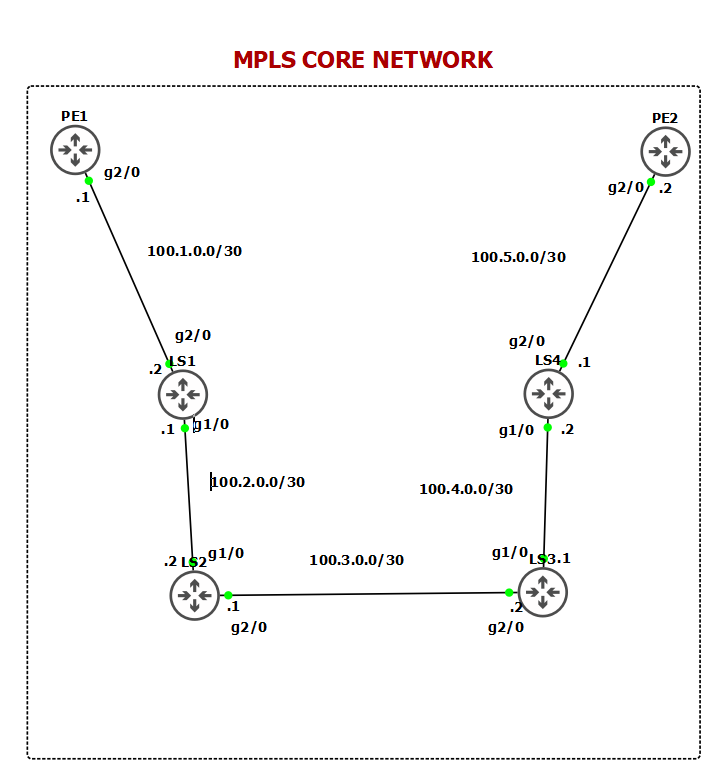
\includegraphics[scale=0.5]{baseMPLS.png}
	\caption{Esquema base de la red MPLS.}
	\label{fig:baseMPLS}
\end{figure}


\textbf{Pregunta 4.}

\textit{Configurar OSPF. Utilice identificador de proceso OSPF 1 ( o con id 1 ), y, área OSPF 0. Anuncie, es decir, incluya las redes conectadas y las de loopback como redes en OSPF. ¿Qué comandos ha usado para configurar OSPF? Indique sólo en un router PE y en un router LS.}

\textit{-Ponga también una captura de show ip route en PE1 para comprobar que OSPF está funcionando.}


\newpage
\begin{lstlisting}[language=bash, caption={Configuración OSPF en el Router PE1}]
    interface Loopback0
     ip address 2.2.2.2 255.255.255.255
     no shutdown
     exit
    
    router ospf 1
     router-id 2.2.2.2
     network 100.1.0.0 0.0.0.3 area 0
     network 2.2.2.2 0.0.0.0 area 0
     exit
\end{lstlisting}

\begin{lstlisting}[language=bash, caption={Configuración OSPF en el Router LS1}]
    interface Loopback0
     ip address 100.1.1.1 255.255.255.255
     no shutdown
     exit
    
    router ospf 1
     router-id 100.1.1.1
     network 100.1.0.0 0.0.0.3 area 0
     network 100.2.0.0 0.0.0.3 area 0
     network 100.1.1.1 0.0.0.0 area 0
     exit
\end{lstlisting}

\begin{figure}[H]
	\centering
	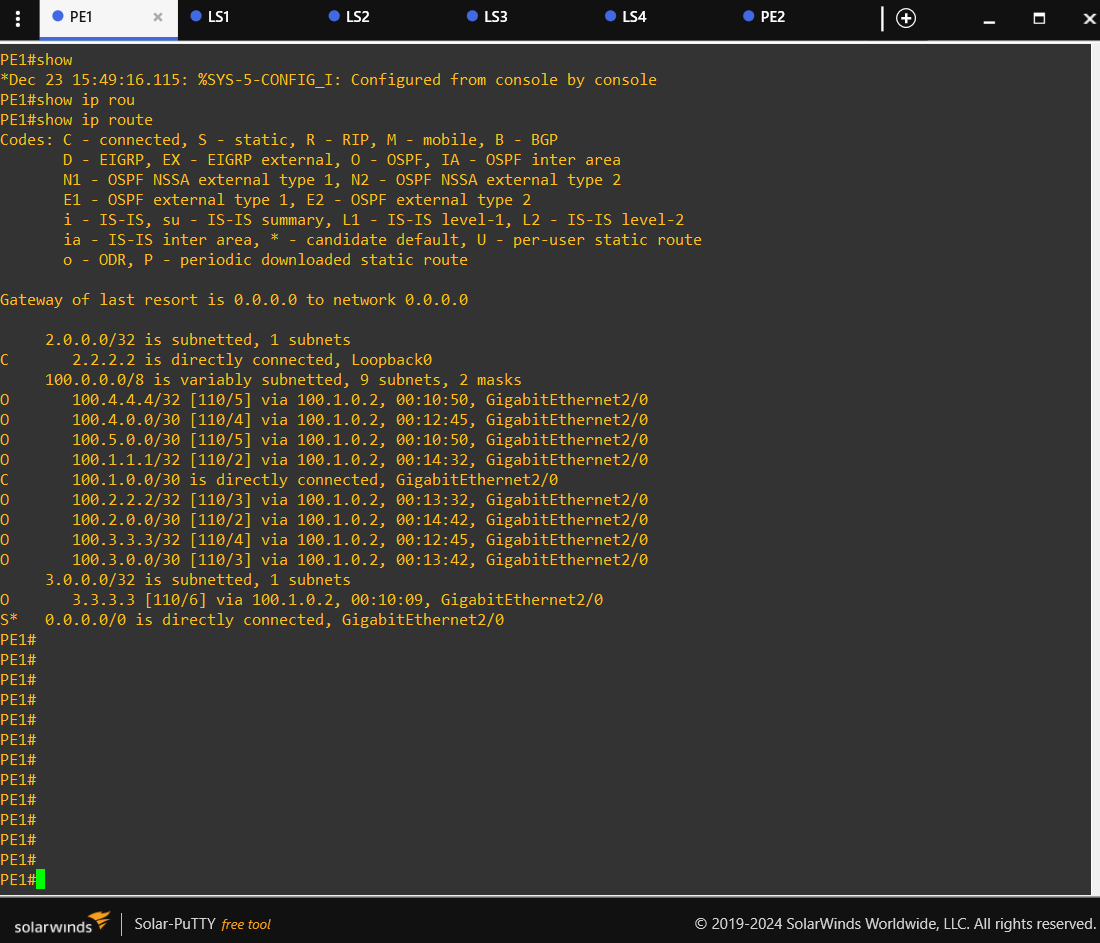
\includegraphics[scale=0.4]{showiproutePE1.png}
	\caption{Captura del comando "show ip route" del router PE1.}
	\label{fig:showiproutePE1}
\end{figure}

\newpage
\textbf{Pregunta 5.}

\textit{Configurar MPLS en cada router de la red CORE. Puede hacerlo de dos formas:}

\textit{• Como en clase, usando mpls ip en cada interfaz de la red mpls, o}

\textit{• Dentro de la configuración OSPF, usando mpls ldp autoconfig . Esta forma es mejor; incluye en MPLS todas las interfaces del router que participen en OSPF, p. ej., añadir nuevas interfaces y no hará falta poner mpls ip para integrarlo en la red MPLS.}

\textit{Indique cuál de las dos alternativas ha usado. Para comprobar que está configurado ponga una
captura de la tabla LFIB (Label Forwarding Information Base, o tabla de forwarding de MPLS) del
router LS1 y del router PE1.}

Se ha optado por configurar MPLS de forma automática usando \texttt{mpls ldp autoconfig}
\begin{figure}[H]
	\centering
	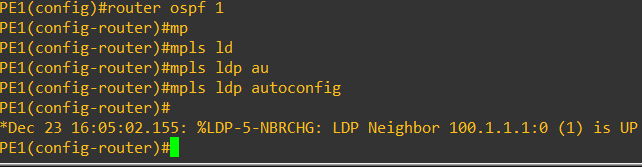
\includegraphics[scale=0.8]{mplsautoconfig.png}
	\caption{Configuración utilizada para configurar MPLS.}
	\label{fig:mplsautoconfig}
\end{figure}

\begin{figure}[H]
	\centering
	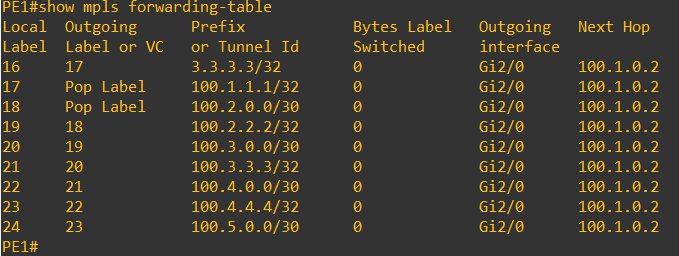
\includegraphics[scale=0.8]{forwardingtablepe1.png}
	\caption{Tabla forwarding del router PE1.}
	\label{fig:forwardingtablepe1}
\end{figure}

\begin{figure}[H]
	\centering
	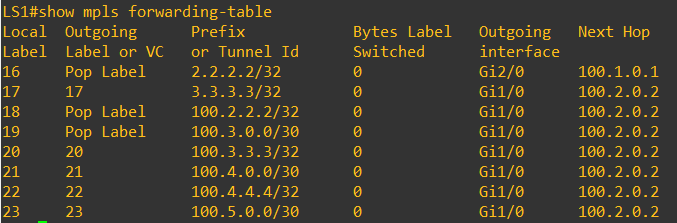
\includegraphics[scale=0.8]{forwardingtablels1.png}
	\caption{Tabla forwarding del router LS1.}
	\label{fig:forwardingtablels1}
\end{figure}

\textbf{Pregunta 6.}
\textit{Compruebe la conectividad. Para ello, incluya las capturas de PINGs}
\begin{figure}[H]
	\centering
	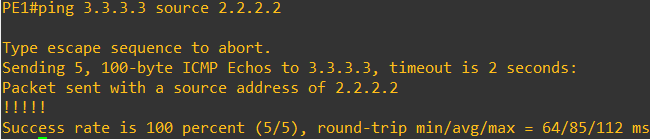
\includegraphics[scale=0.8]{pingpe1pe2.png}
	\caption{Ping exitoso entre los Loopbacks de PE1 y PE2.}
	\label{fig:pingpe1pe2}
\end{figure}

\begin{figure}[H]
	\centering
	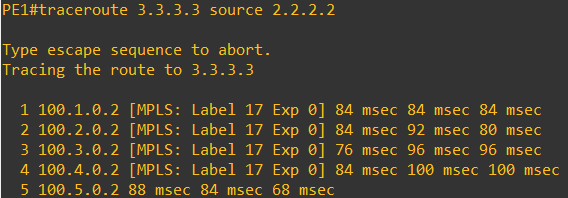
\includegraphics[scale=0.8]{traceroutepe1pe2.png}
	\caption{Traceroute entre los Loopbacks de PE1 y PE2.}
	\label{fig:traceroutepe1pe2}
\end{figure}

\begin{figure}[H]
	\centering
	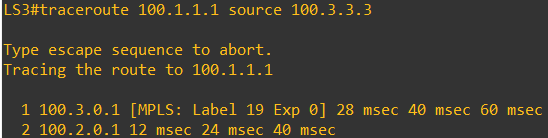
\includegraphics[scale=0.8]{traceroutels3ls1.png}
	\caption{Traceroute entre los Loopbacks de LS3 y LS1.}
	\label{fig:traceroutels3ls1}
\end{figure}

\begin{figure}[H]
	\centering
	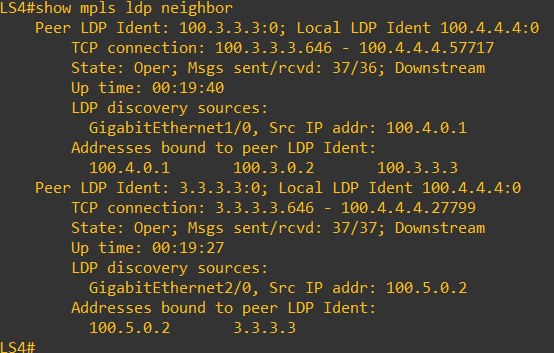
\includegraphics[scale=0.8]{neighborls4.png}
	\caption{Routers vecinos del router LS4.}
	\label{fig:neighborls4}
\end{figure}
\newpage

\section{\texttt{Ejercicio 2.  MP-BGP}}

\textit{Establezca una sesión iBGP (a.k.a. Multiprotocol BGP, MP-BGP) entre PE1 y PE2. Esto nos va a permitir anunciar las rutas VRF entre los dos PEs. MP-BGP sólo va a ejecutar en los PEs, y sólo debe tratar con las rutas de los VRFs de cada cliente.}

\textbf{Pregunta 1.}
\textit{En la consola de PE1, configure BGP. Compruebe que las direcciones fuente de las
conexiones BGP corresponden a las interfaces de Loopback. Para ello}

\textit{• Configure el neighbor usando la IP de loopback del router PE2 distante, indicando el
remote-as 65100 (observe que el neighbor está dentro del mismo AS y, por tanto, es iBGP),
y,}

\textit{• Configure el neighbor de esa dirección de loopback del router remoto añadiendo “update-
source loopback 0”}

\textit{De esa forma la fuente de los paquetes será la dirección de Loopback del PE2}

Para establecer una sesión BGP entre PE1 hasta PE2 se ha añadido la siguiente configuración para PE1:
\begin{lstlisting}[language=bash, caption={Configuración OSPF en el Router LS1}]
router bgp 65100
 bgp log-neighbor-changes
 neighbor 3.3.3.3 remote-as 65100
 neighbor 3.3.3.3 update-source Loopback0
\end{lstlisting}

\textbf{Pregunta 2.}
\textit{Ahora, hay que transportar los prefijos de las redes de mis clientes. Debe configurar en BGP
una address-family y activarla. Dentro de la configuración BGP
address-family vpnv4. Este tipo de address family es el usado normalmente en redes
MPLS donde el forwarding se hace basado en labels.}

\textit{neighbor 3.3.3.3 activate}

\textit{Nótese que usamos sólo una address-family vpnv4 para los dos clientes A y B, ya que usamos
sólo una sesión BGP para transportar los prefijos de los dos clientes.}

Se han implementado los \texttt{address-family} con las siguientes líneas de configuración dentro del \texttt{router bgp 65100}:

\begin{lstlisting}[language=bash, caption={Configuración OSPF en el Router LS1}]
    address-family vpnv4
    neighbor 3.3.3.3 activate
    neighbor 3.3.3.3 send-community extended
   exit-address-family
\end{lstlisting}

\textbf{Pregunta 3.}
\textit{Repita la configuración dual, del protocolo BGP en el router PE2, de forma que este router
establezca un relación BGP con PE1}

Del mismo modo se  completaría para PE2 solo que reemplazando la dirección remota a \texttt{2.2.2.2}.
\newpage
\textbf{Pregunta 4.}
\textit{Comprobación:}

Al realizar el comando \texttt{show bgp vpnv4 unicast all summary}:
\begin{figure}[H]
	\centering
	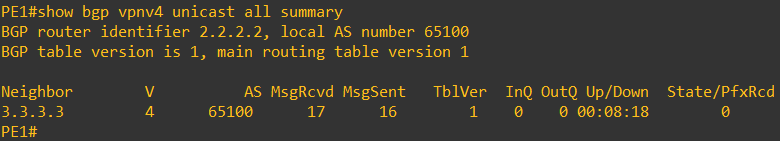
\includegraphics[scale=0.7]{bgppe1.png}
	\caption{Resultado "show bgp" en PE1.}
	\label{fig:bgppe1}
\end{figure}

\begin{figure}[H]
	\centering
	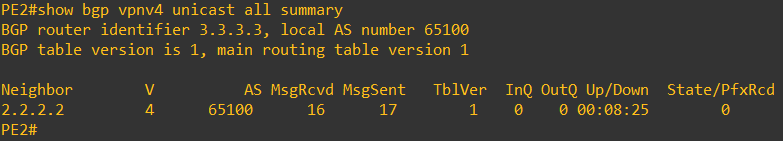
\includegraphics[scale=0.7]{bgppe2.png}
	\caption{Resultado "show bgp" en PE2.}
	\label{fig:bgppe2}
\end{figure}

\newpage
\section{\texttt{Ejercicio 3. VRF}}

\textit{Hay que crear un VRF, Virtual Routing and Forwarding, para cada cliente, A y B, y, en cada uno de los router PE.}

\textbf{Pregunta 1.}
\textit{
	En GNS3, añada y conecte a la red MPLS, los routers de los dos clientes, A y B, y en los dos
sites, tal y como se muestra en la figura/esquema inicial. Es decir, conectar routers CE-A1 y
CE-B1 a PE1, y, routers CE-A2 y CE-B2 a PE2
}

\begin{figure}[H]
	\centering
	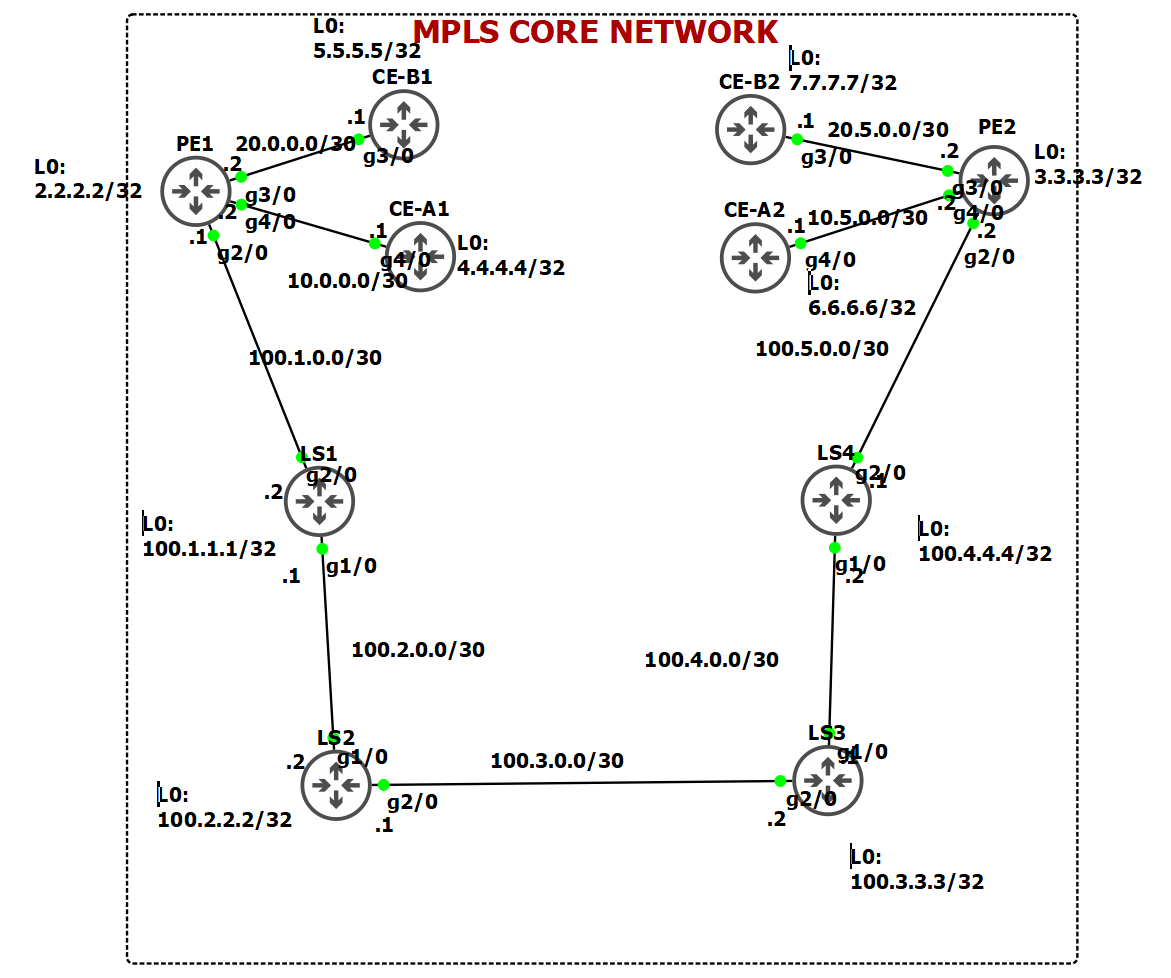
\includegraphics[scale=0.5]{maqueta2.png}
	\caption{Esquema tras agregar los clientes A y B.}
	\label{fig:maqueta2}
\end{figure}
\newpage
\textbf{Pregunta 2.}
\textit{Configure las IPs/mascara de las tres interfaces GigabitEthernet de CE-A1 (+ loopback), y, las
tres interfaces de CE-B1 (+ loopback). Hágalo también con los routers CEs del Site 2, es decir
con los routers CE-A2 y CE-B2. No configure aún las IPs de los routers PEs que conectan
con los clientes.}

\begin{lstlisting}[language=bash, caption={Configuración IPs en el Router CE-A1}]
    interface GigabitEthernet4/0
    ip address 10.0.0.1 255.255.255.252
    no shutdown
    exit
    interface GigabitEthernet2/0
    ip address 172.16.2.1 255.255.255.0
    no shutdown
    exit
    interface FastEthernet0/0
    ip address 172.16.1.1 255.255.255.0
    no shutdown
    exit
	interface Loopback0
    ip address 4.4.4.4 255.255.255.255
    no shutdown
    exit
\end{lstlisting}

\textbf{Pregunta 3.}
\textit{Configure el protocolo OSPF en los 4 routers CEs de los clientes, incluyendo o anunciando
las tres redes conectadas por las interfaces GigabitEthernet y la red de la interfaz Loopback.
Use el ID de proceso OSPF 1 y el area 2, en los 2 routers del cliente A, CE-A1 y CE-A2.
Use el ID de proceso OSPF 1 y el area 4, en los 2 routers del cliente B, CE-B1 y CE-B2.}

\begin{lstlisting}[language=bash, caption={Configuración OSPF en el Router CE-A1}]
    router ospf 1
    router-id 4.4.4.4
    network 172.16.1.0 0.0.0.255 area 2
    network 172.16.2.0 0.0.0.255 area 2
    network 10.0.0.0 0.0.0.3 area 2
    network 4.4.4.4 0.0.0.0 area 2
    mpls ldp autoconfig --quitar
\end{lstlisting}
\newpage
\textbf{Pregunta 4.}
\textit{Comprobaciones previas a configurar VRF. En el router PE1, realice “show mpls interfaces”, “show mpls ldp neighbor”, debe mostrar sólo un peer; “show ip ospf neighbor”, sólo debe tener un vecino OSPF (LS1).}

\textit{Resultados similares debe obtener en el router PE2.}

Puesto que aun no hemos configurado las interfaces hacia los clientes A y B, el router PE1 no conoce de los routers vecinos A y B

\begin{figure}[H]
	\centering
	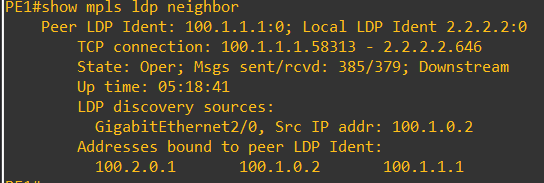
\includegraphics[scale=0.7]{neighborpe1.png}
	\caption{Resultado "show mpls interfaces" en PE1.}
	\label{fig:neighborpe1}
\end{figure}

\begin{figure}[H]
	\centering
	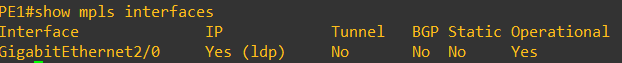
\includegraphics[scale=0.7]{showmplspe1.png}
	\caption{Resultado "show mpls ldp neighbor" en PE1.}
	\label{fig:showmplspe1}
\end{figure}

\begin{figure}[H]
	\centering
	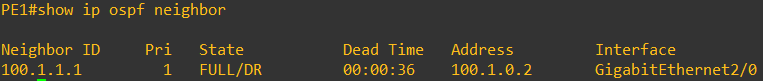
\includegraphics[scale=0.7]{ospfneighborpe1.png}
	\caption{Resultado "show ip ospf neighbor" en PE1.}
	\label{fig:ospfneighborpe1}
\end{figure}

\textbf{Pregunta 5.}
\textit{ Desde la consola de PE1, cree un VRF, Virtual Routing and Forwarding, para el cliente A con
los siguientes parámetros:}


\textit{Nombre del vrf: CUST-A}

\textit{• Router distinguisher con formato AS:nn, es decir, 65100:11, donde ‘nn=11’ es el
identificador del cliente A. Nota: El RD se une al prefijo IP para distinguir clientes
dentro del AS de forma que dos clientes diferentes del operador tengan las mismas
IPs.}

\textit{• Router target (rt) con opción ‘both’ para tener en cuenta tanto los prefijos CIDR
entrantes como los salientes de la red. Para el cliente A daremos el mismo formato e
identificador, 65100:11 . El RT sirve a nivel de datos para ordenar las rutas.
Configuraciones de importación/exportación de rutas entre Sites pueden ajustarse de
detalladamente con RT de exportación e importación diferentes. Nosotros vamos a
simplificar importando/exportando (opción both) el mismo RT para cada cliente.
7}


\textit{Cree un segundo VRF para el segundo cliente del proveedor, Cliente B, y con el
nombre de vrf CUST-B . Respecto al router distinguisher y router target puede usar
65100:22}

\textit{Debe asignar las interfaces que conectan con los routers de los clientes A y B a cada
uno de los VRFs que ha creado. Para ello, por ejemplo, para el cliente A, entramos en
la configuración de g0/0 y usamos “ip vrf forwarding CUST-A”. Dualmente para el
cliente B (CUST-B) en g1/0.}

\textit{Una vez que ha hecho esto, debe configurar la dirección IP y máscara de las dos
interfaces del router PE1 que acaba de configurar, es decir, g0/0 y g1/0. Por supuesto,
haga no shutdown de dichas interfaces.
}

\begin{lstlisting}[language=bash, caption={Comandos utilizados para crear la VRF CUST-A de PE1}]
    ip vrf CUST-A
	rd 65100:11
	route-target both 65100:11
	exit
\end{lstlisting}

\texttt{Para crear la VRF de CUST-B se ha seguido el mismo procedimiento pero reemplazando 65100:11 por 65100:22}

\begin{lstlisting}[language=bash, caption={Comandos utilizados para asignar la VRF CUST-A a la interfaz correspondiente en PE1}]
	interface GigabitEthernet4/0
	ip vrf forwarding CUST-A
	ip address 10.0.0.2 255.255.255.252
	no shutdown
\end{lstlisting}

\begin{lstlisting}[language=bash, caption={Comandos utilizados para asignar la VRF CUST-B a la interfaz correspondiente en PE1}]
	interface GigabitEthernet3/0
	ip vrf forwarding CUST-B
	ip address 20.0.0.2 255.255.255.252
	no shutdown
\end{lstlisting}

\textbf{Pregunta 6.}
\textit{Repita el punto 5, la creación de los 2 VRFs, uno para cada cliente, ahora, en el
router PE2 . Nota: debe usar, como es lógico, el mismo distinguisher y target que ha usado en
cada cliente en el router PE1.}

\begin{lstlisting}[language=bash, caption={Comandos utilizados para asignar la VRF CUST-A a la interfaz correspondiente en PE1}]
	interface GigabitEthernet4/0
	ip vrf forwarding CUST-A
	ip address 10.5.0.2 255.255.255.252
	no shutdown
\end{lstlisting}

\begin{lstlisting}[language=bash, caption={Comandos utilizados para asignar la VRF CUST-B a la interfaz correspondiente en PE1}]
	interface GigabitEthernet3/0
	ip vrf forwarding CUST-B
	ip address 20.5.0.2 255.255.255.252
	no shutdown
\end{lstlisting}
\textbf{Pregunta 7.}
\textit{Por último, como comprobación, podemos realizar:}

\textit{• En PE1: “ping vrf CUST-A 10.0.0.1”}

\textit{• En PE2: “ping vrf CUST-B 20.5.0.1”}

\textit{• En PE2: “show ip vrf interface”}

\begin{figure}[H]
	\centering
	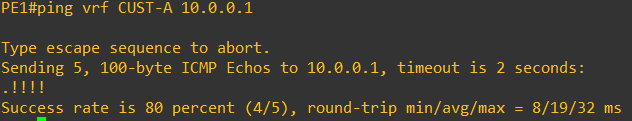
\includegraphics[scale=0.7]{vrfpingpe1.png}
	\caption{Resultado de "ping vrf CUST-A 10.0.0.1".}
	\label{fig:vrfpingpe1}
\end{figure}

\begin{figure}[H]
	\centering
	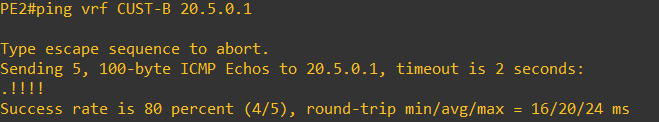
\includegraphics[scale=0.7]{vrfpingpe2.png}
	\caption{Resultado de "ping vrf CUST-B 20.5.0.1".}
	\label{fig:vrfpingpe2}
\end{figure}
\begin{figure}[H]
	\centering
	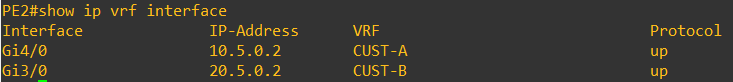
\includegraphics[scale=0.7]{showipvrf.png}
	\caption{Resultado de "show ip vrf interface".}
	\label{fig:showipvrf}
\end{figure}
\textbf{Pregunta 8.}
\textit{El cliente A y el cliente B tienen direcciones de red diferentes en los dos sites. ¿Podrían tener
el mismo direccionamiento, es decir, usar el mismo rango de IPs?, ¿por qué?.}

Sí sería posible debido a que VRF es capaz de diferenciar las redes gracias a técnicas empleadas como Router Distinguisher que añade un prefijo único por cliente gracias a la configuración realizada en Router target (RT).
\newpage

\section{\texttt{Ejercicio 4. Intercambio de rutas entre proveedor y clientes}}

\textit{En los ejercicios anteriores hemos configurado protocolos de encaminamiento en las redes de los
clientes A y B en los dos Sites. También, el proveedor de servicio utiliza un protocolo de
encaminamiento para crear y distribuir sus rutas internas entre los routers que componen la red
core/MPLS. En este ejercicio hemos usado OSPF dentro de la red MPLS (aunque se podría usar
cualquier IGP).
En este ejercicio debe configurar el intercambio de rutas entre los routers CEs y los PEs.
Como en los routers PEs, cada cliente tiene tablas de encaminamiento (VRF) independientes,
debemos crear un proceso OSPF asociado con el VRF del cliente A y otro proceso OSPF
asociado al VRF del cliente B, y, a añadir (usando network) la red que conecta con el router CE
del cliente en cuestión. Los id’s de los procesos OSPF que configuremos para cada cliente
deben tener un pid, “número del proceso OSPF” diferente que el que usa el PE, para
intercambiar rutas dentro de la red core MPLS.}
\newpage
\textbf{Pregunta 1.}
\textit{
	Comprobación previa:
}

\textit{
	En CE-A1 obtenga la información de OSPF que hizo con anterioridad.
}

\textit{En PE1 haga PING a la dirección 10.0.0.1 de la tabla VRF CUST-A}

\textit{En PE1 del mismo modo intente hacer PING a la interfaz de loopback de CE-A1}

\textit{En PE1, ¿llegan los dos PINGs?. Si no llega alguno de los PINGs ¿por qué cree que sucede
esto?}

\begin{figure}[H]
	\centering
	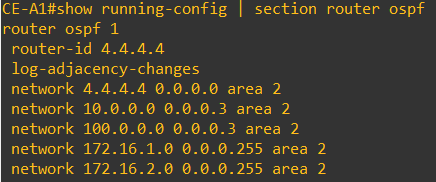
\includegraphics[scale=0.7]{ospfconfigcea1.png}
	\caption{Resultado de "show running-config | section router ospf" en CE-A1.}
	\label{fig:ospfconfigcea1}
\end{figure}

\begin{figure}[H]
	\centering
	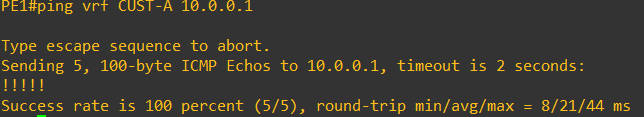
\includegraphics[scale=0.7]{vrfpingpe1-segundo.png}
	\caption{Resultado del ping VRF de PE1 a CE-A1 de nuevo.}
	\label{fig:vrfpingpe1-segundo}
\end{figure}

\begin{figure}[H]
	\centering
	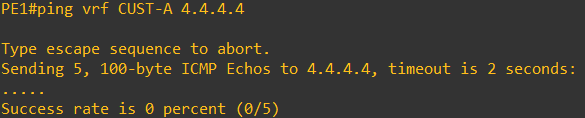
\includegraphics[scale=0.7]{pingVRFtoLoopback.png}
	\caption{Resultado del ping VRF de PE1 al Loopback0 de CE-A1.}
	\label{fig:pingVRFtoLoopback}
\end{figure}

Como podemos apreciar, el ping VRF al Loopback no puede realizarse, muy probablemente se debe a que PE1 desconoce de la red del Loopback0 de CE-A1 ya que esta no ha sido anunciada aún.
\newpage
\textbf{Pregunta 2.}
\textit{En la consola del router PE1,}

\textit{Para el cliente A (vrf CUST-A) crearemos un proceso OSPF con id 2 y añadiremos la red
10.0.0.0 con el wildcard que corresponde a esa red, y, usaremos area 2}

\textit{Para el cliente B (vrf CUST-B) crearemos un proceso OSPF con id 3 y añadiremos la red
20.0.0.0 con el wildcard que corresponde a esa red, y, usaremos area 4}


\begin{lstlisting}[language=bash, caption={Configuración en PE1 para recibir las Loopbacks de los clientes}]
	configure terminal
	router ospf 2 vrf CUST-A
	 router-id 10.0.0.2
	 network 10.0.0.0 0.0.0.3 area 2
	exit
	configure terminal
router ospf 3 vrf CUST-B
 router-id 20.0.0.2
 network 20.0.0.0 0.0.0.3 area 4
exit
\end{lstlisting}
\newpage
\textbf{Pregunta 3.}
\textit{En la consola del router PE2,}

\textit{Realice la misma configuración de dos procesos OSPF (id 2 area 2, e, id 3 area 4) y
anuncie las rutas que le conectan con CE-A2 y CE-B2, añadiendo las redes 10.5.0.0 y
20.5.0.0.}

\textit{Comprobación final:}

\textit{• Realice un PING a la IP 7.7.7.7}

\textit{• Muestre la tabla de encaminamiento de CUST-A. En la salida del comando debería ver
las rutas hacia las redes de ese cliente.}

\begin{lstlisting}[language=bash, caption={Configuración en PE2 para recibir las Loopbacks de los clientes}]
	configure terminal
	router ospf 2 vrf CUST-A
	 router-id 10.5.0.2
	 network 10.5.0.0 0.0.0.3 area 2
	exit
	configure terminal
router ospf 3 vrf CUST-B
 router-id 20.5.0.2
 network 20.5.0.0 0.0.0.3 area 4
exit
\end{lstlisting}

Tras haber realizado la configuración previa, ahora los routers PE sí son capaces de realizar pings a los Loopbacks de los clientes.

\begin{figure}[H]
	\centering
	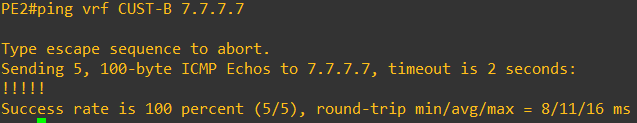
\includegraphics[scale=0.7]{pingloopbackexito.png}
	\caption{Resultado del ping VRF de PE2 al Loopback0 7.7.7.7.}
	\label{fig:pingloopbackexito}
\end{figure}
\newpage
\section{\texttt{Ejercicio 5. Redistribución de rutas}}
\textit{Como resultado de los ejercicios anteriores tenemos:}

\textit{• Una red MPLS configurada que nos sirve de red de transporte}

\textit{• Routers frontera, PE, que reciben información de encaminamiento de las redes de sus clientes,
y, además, de forma independiente, es decir distinguiendo la información recibida de cada uno.}

\textit{• Una sesión BGP establecida entre los routers PEs que permite enviar las rutas de los clientes
de un extremo a otro de la red core/MPLS}

\texttt{REDISTRIBUCIÓN DE OSPF EN BGP:}

Nos resta redistribuir las rutas que recibimos de los routers CE de los clientes en el protocolo
BGP. Esto va a permitir que las rutas de cada cliente asociadas a cada VRF se transporten del
PE1 al PE2, y viceversa.

\textbf{Pregunta 1.}
\textit{En el router PE1:}

\textit{Comprobación inicial:}

\textit{• “show ip bgp vpnv4 vrf CUST-A”}

\textit{• “show ip bgp vpnv4 vrf CUST-B”}

\textit{Todavía no hemos hecho la redistribución y, por tanto, no deben salir rutas.}

\begin{figure}[H]
	\centering
	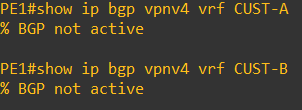
\includegraphics[scale=1]{showipbgp.png}
	\caption{Resultado del comando "show ip bgp vpnv4 vrf ---" para cada cliente.}
	\label{fig:showipbgpCUSTA}
\end{figure}

Este resultado en mi caso se trata de un error debido a una mala configuración previa, el resultado ha de ser vacío.
\newpage
\textbf{Pregunta 2.}
\textit{Redistribuir rutas OSPF en BGP. Debe redistribuir las rutas que le llegan de los dos clientes A
y B a través de la red MPLS.}

\textit{Para realizar la redistribución, en la consola de PE1 debe}

\textit{• Entrar en la configuración de bgp del sistema autónomo, 65100.}

\textit{• Seguidamente, entrar en address-family command mode, en este caso, tipo de familia
ipv4, y, vrf, primero para el CUST-A.}

\textit{• Realizar redistribute del proceso ospf que asignó al cliente A (ospf 2).}

\textit{• Con esto ya ha redistribuido las rutas de OSPF a BGP para el CUST-A. Debe hacer, de
forma dual, la redistribución para el CUST-B.}

\begin{lstlisting}[language=bash, caption={Configuración de bgp en PE1}]
router bgp 65100
 address-family ipv4 vrf CUST-A
  redistribute ospf 2
 exit-address-family
exit
router bgp 65100
 address-family ipv4 vrf CUST-B
  redistribute ospf 3
 exit-address-family
exit
\end{lstlisting}
\textbf{Pregunta 3.}
\textit{
	Repitiendo los comandos show… del punto 1. ¿Qué observa?
Al observar las rutas BGP de los VRF de cada cliente aún no podemos ver las rutas del site
remoto (site 2). Para verlas debemos configurar la redistribución en el otro router PE, en PE2.
}
\begin{figure}[H]
	\centering
	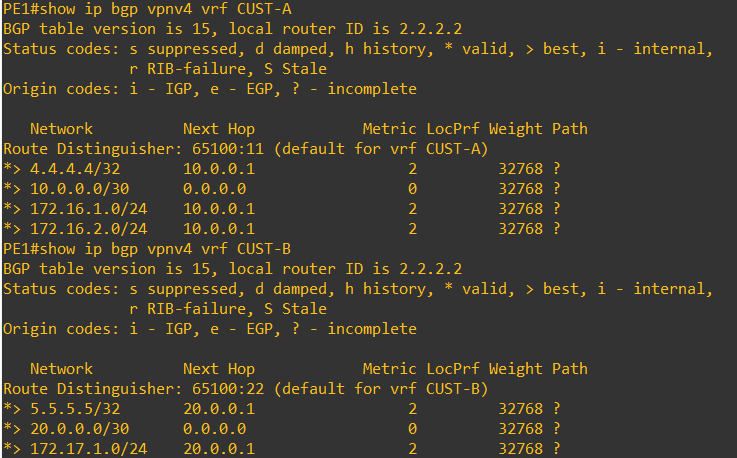
\includegraphics[scale=0.7]{showipbgpNUEVO.png}
	\caption{Resultado del comando "show ip bgp vpnv4 vrf ---" para cada cliente.}
	\label{fig:showipbgpNUEVO}
\end{figure}

\textbf{Pregunta 4.}
\textit{
	En la consola de PE2 realice la redistribución de rutas OSPF en BGP, tal y como hizo en el
punto 2. anterior para el router PE1.
}

\begin{lstlisting}[language=bash, caption={Configuración de bgp en PE2}]
router bgp 65100
 address-family ipv4 vrf CUST-A
  redistribute ospf 2
 exit-address-family
exit
router bgp 65100
 address-family ipv4 vrf CUST-B
  redistribute ospf 3
 exit-address-family
exit
\end{lstlisting}

\textbf{Pregunta 5.}
\textit{ Comprobación:}
\textit{En PE1 vea las rutas que ha redistribuido de los clientes en BGP:}

\textit{• “show ip bgp vpnv4 vrf CUST-A”}

\textit{• “show ip bgp vpnv4 vrf CUST-B”}


\textit{Las IPs que tengan la ‘i’ son rutas que se ha redistribuido del mismo cliente desde el site
remoto (site 2). Realice la misma comprobación en PE2
}

Tras haber configurado PE2, obtenemos ya las redes remotas:

\begin{figure}[H]
	\centering
	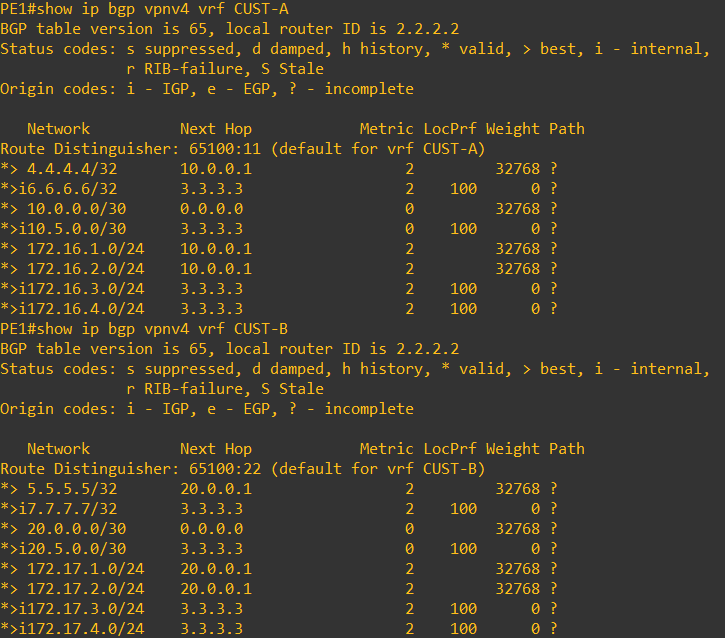
\includegraphics[scale=0.6]{showipbgpNUEVOPE1.png}
	\caption{Resultado del comando "show ip bgp vpnv4 vrf ---" para cada cliente.}
	\label{fig:showipbgpNUEVOPE1}
\end{figure}

\begin{figure}[H]
	\centering
	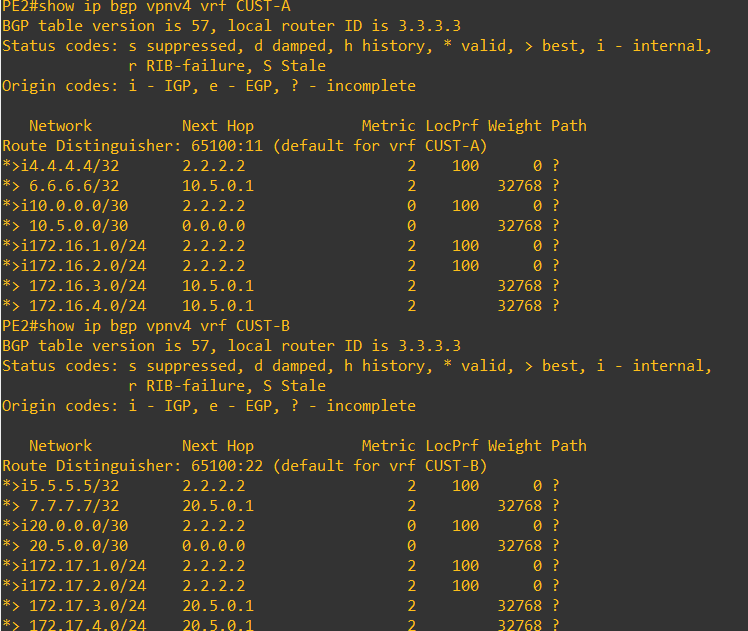
\includegraphics[scale=0.6]{showipbgpNUEVOPE2.png}
	\caption{Resultado del comando "show ip bgp vpnv4 vrf ---" para cada cliente.}
	\label{fig:showipbgpNUEVOPE2}
\end{figure}


\textit{
	REDISTRIBUCIÓN DE BGP EN OSPF:
Por último, hay que redistribuir las rutas que se transportan con BGP por la red core/MPLS al
protocolo OSPF que usan los sites de los clientes A y B.
}
\newpage
\textbf{Pregunta 6.}
\textit{En el router PE1:}

\textit{Entre en la configuración de ospf de id de proceso asignado al cliente A. Seguidamente
realice la redistribute de bgp 65100 considerando las subnets.}

\textit{Repita la configuración anterior para el cliente B utilizando el id de proceso ospf que
utilizó para el cliente B en los routers frontera.}

\begin{lstlisting}[language=bash, caption={Configuración añadida de ospf en PE1}]
	router ospf 2 vrf CUST-A
	redistribute bgp 65100 subnets
	exit

	router ospf 2 vrf CUST-B
	redistribute bgp 65100 subnets
	exit
\end{lstlisting}

\textbf{Pregunta 7.}
\textit{Repita la configuración completa del punto 6 anterior en la consola del router PE2.}

\begin{lstlisting}[language=bash, caption={Configuración añadida de ospf en PE2}]
	router ospf 2 vrf CUST-A
	redistribute bgp 65100 subnets
	exit

	router ospf 2 vrf CUST-B
	redistribute bgp 65100 subnets
	exit
\end{lstlisting}

\newpage
\section{\texttt{Ejercicio 6. Comprobación final}}

\textit{Una vez hemos completado los pasos anteriores, debemos tener conectividad entre los routers
CEs de cada cliente, por ejemplo, entre CE-A1 y CE-A2.}

\textbf{Pregunta 1.}
\textit{En la consola de CE-A1:}

\textit{Haga PING a la dirección IP 6.6.6.6 del router CE-A2.}

\textit{Haga “show ip route” para ver la tabla de encaminamiento. Debe observar 4 rutas OSPF
ínter area (O IA) que corresponden con el site remoto del cliente A.}

\textit{Realice un traceroute a la dirección IP 6.6.6.6}

\begin{figure}[H]
	\centering
	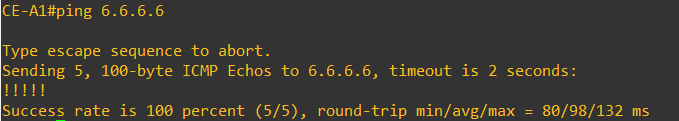
\includegraphics[scale=0.6]{ping6666.png}
	\caption{Resultado del ping CE-A1 al Loopback de CE-A2.}
	\label{fig:ping6666}
\end{figure}

\begin{figure}[H]
	\centering
	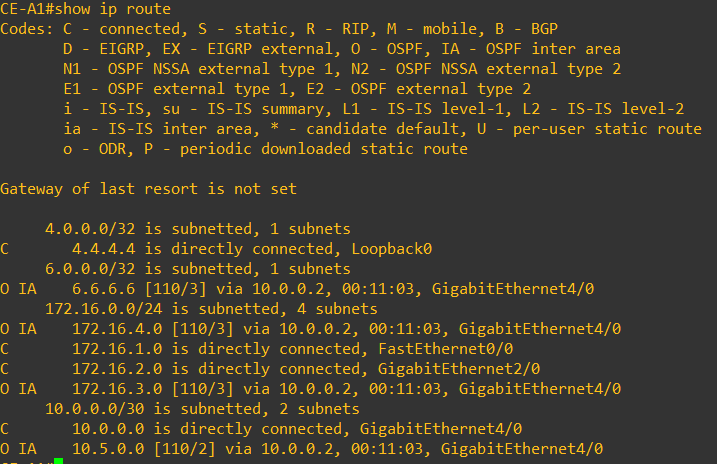
\includegraphics[scale=0.6]{showiproutea1.png}
	\caption{Resultado del Ip Route CE-A1.}
	\label{fig:showiproutea1}
\end{figure}

\begin{figure}[H]
	\centering
	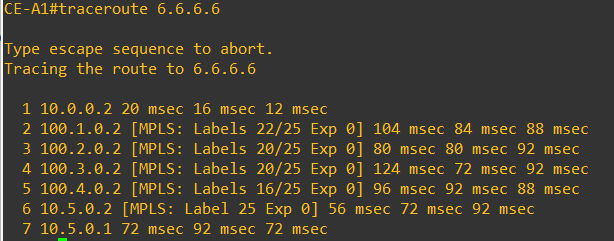
\includegraphics[scale=0.6]{traceroute6666.png}
	\caption{Resultado del Traceroute CE-A1 al Loopback de CE-A2.}
	\label{fig:traceroute6666}
\end{figure}
\newpage
\textbf{Pregunta 2.}
\textit{En la consola de CE-B2:}


\textit{Haga PING a la dirección IP 5.5.5.5 del router CE-B1.}

\textit{Haga “show ip route” para ver la tabla de encaminamiento. Debe observar 4 rutas OSPF
ínter area (O IA) que corresponden con el site remoto del cliente B.}

\textit{Realice un traceroute a la dirección IP 5.5.5.5}

\begin{figure}[H]
	\centering
	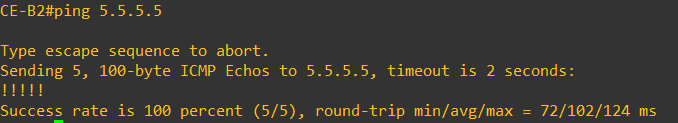
\includegraphics[scale=0.6]{ping5555.png}
	\caption{Resultado del ping CE-B2 al Loopback de CE-B1.}
	\label{fig:ping5555}
\end{figure}

\begin{figure}[H]
	\centering
	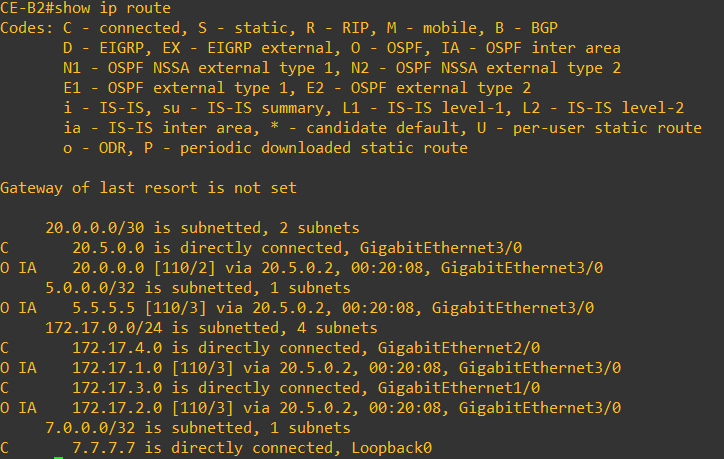
\includegraphics[scale=0.6]{showiprouteb2.png}
	\caption{Resultado del Ip Route CE-B2.}
	\label{fig:showiprouteb2}
\end{figure}

\begin{figure}[H]
	\centering
	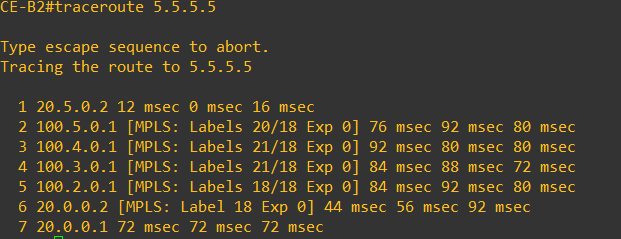
\includegraphics[scale=0.6]{traceroute5555.png}
	\caption{Resultado del Traceroute CE-B2 al Loopback de CE-B1.}
	\label{fig:traceroute5555}
\end{figure}
\newpage
\section{\texttt{Ejercicio 7. Conexión de dos Sites de un tercer cliente de la red MPLS}}

\textit{Ahora que ya tiene conectados dos clientes, conoce lo necesario para extender la red y conectar
un tercer cliente CUST-C tal y como muestra la siguiente figura:}

\begin{figure}[H]
	\centering
	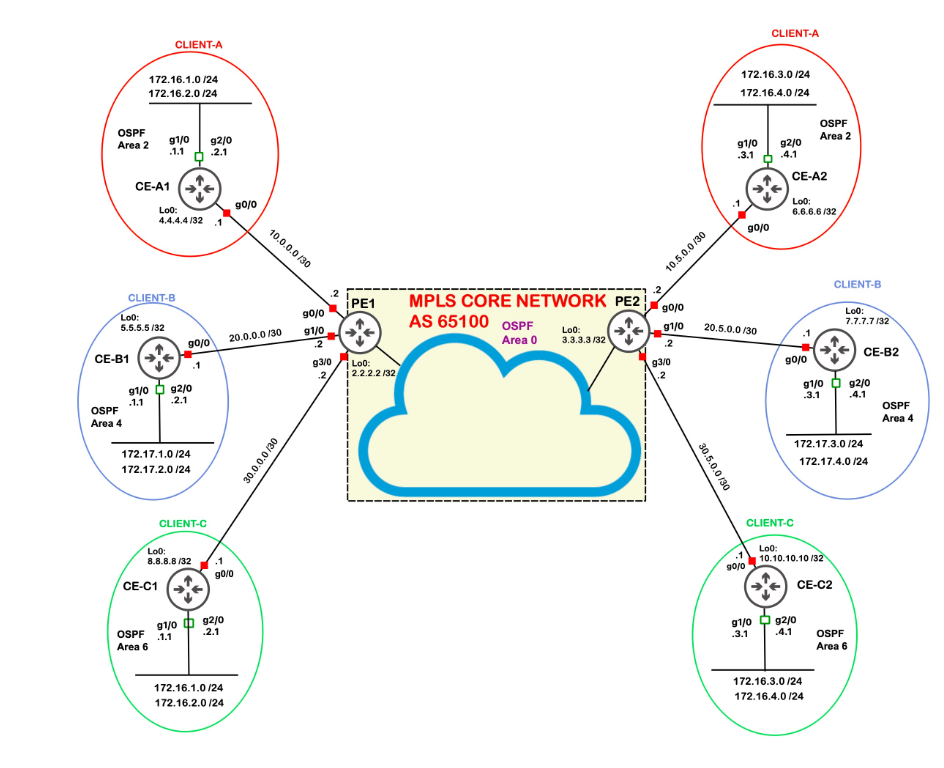
\includegraphics[scale=0.6]{fig3.png}
	\caption{Figura de la maqueta a realizar.}
	\label{fig:fig3}
\end{figure}

\textit{Nota: Las direcciones IP de las subredes de los 2 Sites C coinciden con los del Site A. También
podrían coincidir las IPs de Loopback pero se han puesto diferentes para se vean más claras las
comprobaciones que debe realizar.}

\textit{Realice las comprobaciones del Ejercicio 6 para este cliente.}
\newpage
\textbf{Pregunta 1.}
\textit{Desde la consola de CE-C2:}

\textit{Haga PING a la dirección IP 8.8.8.8 del router CE-C1.}

\textit{Haga “show ip route” para ver la tabla de encaminamiento. Debe observar 4 rutas
OSPF ínter area (O IA) que corresponden con el site remoto del cliente C.}

\textit{Realice un traceroute a la dirección IP 8.8.8.8}

Para realizar este ejercicio, se ha integrado físicamente dos nuevos routers clientes, CE-C1 y CE-C2 como muestra en la siguiente imagen:
\begin{figure}[H]
	\centering
	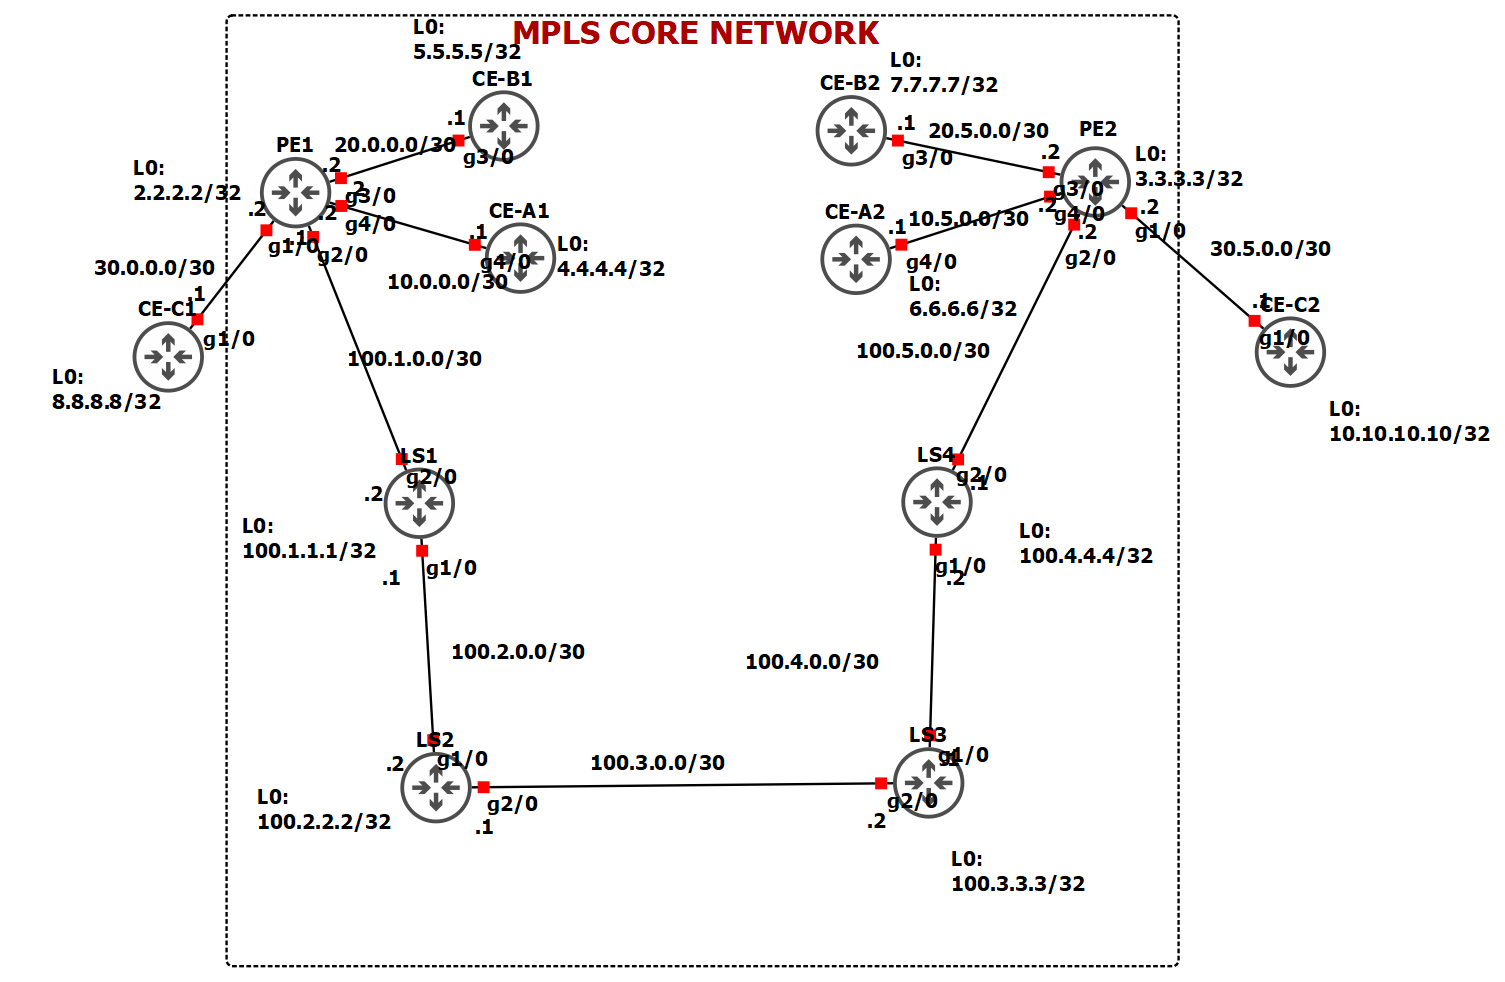
\includegraphics[scale=0.4]{maqueta3.png}
	\caption{Maqueta resultante tras añadir un tercer cliente.}
	\label{fig:maqueta3}
\end{figure}

La configuración realizada es exactamente la misma que en todos los ejercicios anteriores, solo que con nuevo cliente llamado CUST-C ahora.
Tras haber realizado la configuración, la batería de pruebas muestra una conexión con éxito entre ambos clientes nuevos:

\begin{figure}[H]
	\centering
	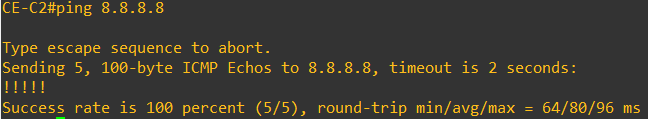
\includegraphics[scale=0.6]{ping8888.png}
	\caption{Resultado del ping CE-C2 al Loopback de CE-C1.}
	\label{fig:ping8888}
\end{figure}

\begin{figure}[H]
	\centering
	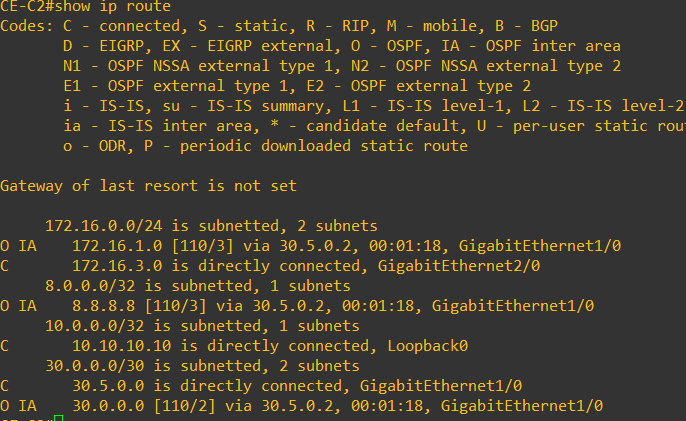
\includegraphics[scale=0.6]{routeipCE.png}
	\caption{Resultado del Ip Route CE-C2.}
	\label{fig:routeipCE}
\end{figure}

\begin{figure}[H]
	\centering
	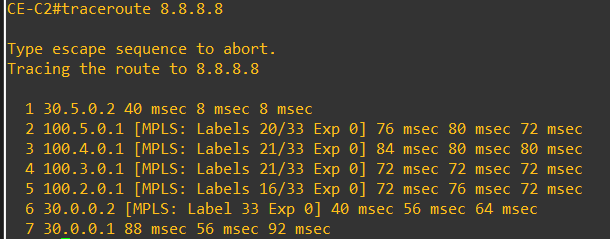
\includegraphics[scale=0.6]{traceroute8888.png}
	\caption{Resultado del Traceroute CE-C2 al Loopback de CE-C1.}
	\label{fig:traceroute8888}
\end{figure}
\appendix
\end{document}
